\section{Benchmark Summary}
For experiments, a total of $752$ kernels ($266$ CUDA and $486$ OpenCL) were considered. This benchmark set is a union of four independent test suites and publicly available \cite{cudatoolkit} sample programs. The source data used to generate this report is available in the $\MB{generated}$ and $\MB{analysis}$ directories. \tableref{benchmark_summary} summarizes the various sources of the kernels.

\section{Benchmark Summary}
For experiments, a total of $752$ kernels ($266$ CUDA and $486$ OpenCL) were considered. This benchmark set is a union of four independent test suites and publicly available \cite{cudatoolkit} sample programs. The source data used to generate this report is available in the $\MB{generated}$ and $\MB{analysis}$ directories. \tableref{benchmark_summary} summarizes the various sources of the kernels.

\section{Benchmark Summary}
For experiments, a total of $752$ kernels ($266$ CUDA and $486$ OpenCL) were considered. This benchmark set is a union of four independent test suites and publicly available \cite{cudatoolkit} sample programs. The source data used to generate this report is available in the $\MB{generated}$ and $\MB{analysis}$ directories. \tableref{benchmark_summary} summarizes the various sources of the kernels.

\section{Benchmark Summary}
For experiments, a total of $752$ kernels ($266$ CUDA and $486$ OpenCL) were considered. This benchmark set is a union of four independent test suites and publicly available \cite{cudatoolkit} sample programs. The source data used to generate this report is available in the $\MB{generated}$ and $\MB{analysis}$ directories. \tableref{benchmark_summary} summarizes the various sources of the kernels.

\input{tables/benchmark_summary}

\section{GPURepair vs. AutoSync Comparison}

\subsection{Result Comparison}
\tableref{results} summarizes the results obtained from running the benchmark suite with \tool and \autosync. The table categorizes the results into three categories based on the output of \verifier. Since \autosync can not take OpenCL kernels as inputs, results for OpenCL is only applicable for \tool. Numbers in bold indicate better results.

For $9$ benchmarks, \autosync stated that the error could not be repaired. Out of these $9$, \tool was able to repair $4$, it timed out for $3$, and it could not repair $2$ of these.

\begin{table}[t]
\caption{Count of kernels grouped by category}
\label{Ta:results}
\centering

\def\arraystretch{1.1}
\setlength\tabcolsep{7pt}

\begin{tabular}{|l|r|r|r|}
\hline

\multicolumn{1}{|c|}{\textbf{Category}} & \multicolumn{1}{|c|}{\textbf{\autosyncname}} & \multicolumn{2}{|c|}{\textbf{\toolname}} \\ \hline
\multicolumn{1}{|c|}{} & \multicolumn{1}{|c|}{\textbf{CUDA}} & \multicolumn{1}{|c|}{\textbf{CUDA}} & \multicolumn{1}{|c|}{\textbf{OpenCL}} \\
\multicolumn{1}{|c|}{Total Benchmarks} & $266$ & $266$ & $486$ \\ \hline \hline
Verified by \verifiername & $152$ & $152$ & $331$ \\ \hline
\quad No changes made by the tool & $146$ & $134$ & $294$ \\
\quad Changes recommended by the tool & $0$ & $\MB{17}$ & $24$ \\
\quad Errors  & $6$ & $\MB{0}$ & $10$ \\
\quad Timeouts & $0$ & $1$ & $3$ \\ \hline \hline

Data Race/Barrier Divergence Errors & \multirow{2}{*}{$89$} & \multirow{2}{*}{$89$} & \multirow{2}{*}{$69$} \\
identified by \verifiername & & & \\ \hline
\quad Repaired by the tool & $31$ & $\MB{55}$ & $30$ \\
\quad Could not be repaired by the tool & $9$ & $22$ & $34$ \\
\quad Errors  & $14$ & $\MB{0}$ & $0$ \\
\quad Timeouts & $35$ & $\MB{12}$ & $5$ \\ \hline \hline

Unrepairable errors identified by & \multirow{2}{*}{$25$} & \multirow{2}{*}{$25$} & \multirow{2}{*}{$86$} \\
\verifiername & & & \\ \hline
\quad Handled gracefully by the tool & $0$ & $\MB{25}$ & $86$ \\
\quad False Positives & $24$ & $\MB{0}$ & $0$ \\
\quad Errors  & $1$ & $\MB{0}$ & $0$ \\ \hline

\end{tabular}
\end{table}


\subsection{Time Comparison}
As described in \tableref{results}, there were $25$ benchmarks in the third category where \verifier itself throws an irreparable error (e.g., either an assertion violation or errors thrown by other stages). We provide a time comparison via the scatter plot shown in \figref{time_scatter_log} for the remaining $241$ benchmarks which are either certified as error free by \verifier or having a presence of data race and/or barrier divergence error.

Out of the $241$ benchmarks, \autosync was faster for $177$ whereas \tool was faster for $64$ benchmarks. Please note that out of these $241$ benchmarks, there are $152$ benchmarks for which \verifier does not show any error. For these benchmarks, \autosync does not have to put any further efforts. On the other hand, \tool attempts to find if there are some programmer inserted barriers that are unnecessary so that they can be removed. \figref{time_repair_log} shows run time comparision for $89$ benchmarks for which \verifier found data-race/barrier divergence errors. \autosync was faster on $31$ benchmarks whereas \tool was faster on $58$ benchmarks out of these $89$ benchmarks. Note that if any of the tools crash on a benchmark, we consider that run to have timed out (e.g., $300$ seconds).

The total time taken for all $241$ benchmarks on average by \autosync is $17302$ seconds whereas \tool takes $6590$ seconds. The median time taken over all the $241$ benchmarks by \autosync is $1.44$ seconds whereas the median time taken by \tool is $1.81$ seconds.

\begin{figure}[htp]
\centering

\begin{minipage}{.45\textwidth}
    \centering
    \begin{tikzpicture}[scale=0.65]
    
    \pgfplotstableread{figures/data/time_scatter.dat}{\data}
    \selectcolormodel{gray}
    
    \begin{axis}[
        xlabel={GPURepair},
        ylabel={AutoSync},
        scaled ticks = false,
        tick label style={
            /pgf/number format/fixed,
            /pgf/number format/precision=3
        },
        xmin=1,
        xmax=300,
        ymin=1,
        ymax=300,
        xmode=log,
        ymode=log,
        log ticks with fixed point
    ]
    
    \addplot[
        scatter=true,
        only marks,
        mark=*,
        scatter src=explicit symbolic,
        scatter/classes={
            a={mark=*}
        }
    ]
    table[x=gpurepair,y=autosync,meta=label]{\data};
    \addplot [black,samples at={0,1}] {x};
    \draw [black,solid] (rel axis cs:0,0) -- (rel axis cs:1,1);
    
    \end{axis}
    \end{tikzpicture}
    \caption{Runtime in seconds (Log Scale)}
    \label{Fi:time_scatter_log}
\end{minipage}
\hskip 10pt
\begin{minipage}{.45\textwidth}
    \centering
    \begin{tikzpicture}[scale=0.65]
    
    \pgfplotstableread{figures/data/time_repaired.dat}{\data}
    \selectcolormodel{gray}
    
    \begin{axis}[
        xlabel={GPURepair},
        ylabel={AutoSync},
        scaled ticks = false,
        tick label style={
            /pgf/number format/fixed,
            /pgf/number format/precision=3
        },
        xmin=1,
        xmax=300,
        ymin=1,
        ymax=300,
        xmode=log,
        ymode=log,
        log ticks with fixed point
    ]
    
    \addplot[
        scatter=true,
        only marks,
        mark=*,
        scatter src=explicit symbolic,
        scatter/classes={
            a={mark=*}
        }
    ]
    table[x=gpurepair,y=autosync,meta=label]{\data};
    \addplot [black,samples at={0,1}] {x};
    \draw [black,solid] (rel axis cs:0,0) -- (rel axis cs:1,1);
    
    \end{axis}
    \end{tikzpicture}
    \caption{Runtime in seconds - Repair Candidates (Log Scale)}
    \label{Fi:time_repair_log}
\end{minipage}

\end{figure}


\subsection{Verifier Calls Comparison}
There were $28$ CUDA kernels that were repaired by both \tool and \autosync. For $129$ CUDA kernels neither \tool nor \autosync suggest any changes. \figref{verifier_calls_all} shows the number of queries made to \verifier by \autosync v/s \tool for all $28+129=157$ kernels which both of them repaired or both of them concurred that no changes are required. The size of the dot is proportional to the number of instances. In total for these $157$ benchmarks, \autosync invoked \verifier $212$ times whereas \tool queried \verifier $294$ times.

\figref{verifier_calls_fixes} provides a comparison to the calls made to the \verifier for only $28$ benchmarks that are repaired by both \tool and \autosync. \tool makes $83$ queries while \autosync makes $137$ calls to \verifier.

\begin{figure}[htp]
\centering

\subfloat[All kernels\label{Fi:verifier_calls_all}]{
    \centering
    
    \pgfplotstableread{figures/data/verifier_calls_all.dat}{\data}
    \begin{tikzpicture}[scale=0.72]
    \selectcolormodel{gray}

    \begin{axis}[
        xlabel={GPURepair},
        ylabel={AutoSync},
        scaled ticks = true,
        tick label style={
            /pgf/number format/fixed,
            /pgf/number format/precision=3
        },
        xmin=0,
        xmax=6,
        ymin=0,
        ymax=6,
    ]

    \addplot[
        scatter=true,
        only marks,
        mark=*,
        point meta=explicit symbolic,
        visualization depends on = {\thisrow{2} \as \perpointmarksize},
        scatter/@pre marker code/.append style={/tikz/mark size=\perpointmarksize},
    ] table [meta index=2] {\data};
    \draw [black,solid] (rel axis cs:0,0) -- (rel axis cs:1,1);

    \end{axis}
    \end{tikzpicture}
}\hfil
\subfloat[Kernels fixed by both tools\label{Fi:verifier_calls_fixes}]{
    \centering
    
    \pgfplotstableread{figures/data/verifier_calls_fixes.dat}{\data}
    \begin{tikzpicture}[scale=0.72]
    \selectcolormodel{gray}

    \begin{axis}[
        xlabel={GPURepair},
        ylabel={AutoSync},
        scaled ticks = true,
        tick label style={
            /pgf/number format/fixed,
            /pgf/number format/precision=3
        },
        xmin=0,
        xmax=6,
        ymin=0,
        ymax=6,
    ]

    \addplot[
        scatter=true,
        only marks,
        mark=*,
        point meta=explicit symbolic,
        visualization depends on = {\thisrow{2} \as \perpointmarksize},
        scatter/@pre marker code/.append style={/tikz/mark size=\perpointmarksize},
    ] table [meta index=2] {\data};
    \draw [black,solid] (rel axis cs:0,0) -- (rel axis cs:1,1);

    \end{axis}
    \end{tikzpicture}
}

\caption{Calls to the Verifier}
\label{Fi:verifier_calls}

\end{figure}


\section{Source Code Information}

\figref{code_lines} shows the size of the kernels in terms of lines of code. The average number of lines of code for the $752$ kernels in the evaluation set was $17.67$, and the median was $11$. $14$ kernels had more than $100$ lines of code, and $47$ had more than $50$ lines of code. $50\%$ of the kernels had less than $25$ lines of code. The kernel with the highest number of lines of code had $639$ lines.

\begin{figure}[htp]
\centering

\begin{minipage}{.45\textwidth}
    \centering
    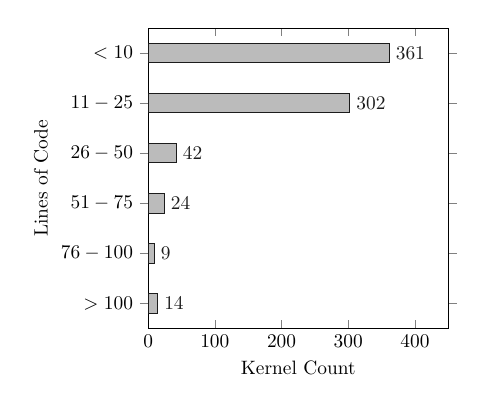
\begin{tikzpicture}[scale=0.7]
    
    \selectcolormodel{gray}
    
    \begin{axis}[
        xbar, xmin=0, xmax=450,
        xlabel={Kernel Count},
        symbolic y coords={
            {$> 100$},
            {$76-100$},
            {$51-75$},
            {$26-50$},
            {$11-25$},
            {$< 10$}
        },
        ytick=data,
        ylabel={Lines of Code},
        nodes near coords,
        nodes near coords align={horizontal},
        height=200pt, width=200pt
    ]
    
    \addplot coordinates {
        (14,{$> 100$})
        (9,{$76-100$})
        (24,{$51-75$})
        (42,{$26-50$})
        (302,{$11-25$})
        (361,{$< 10$})
    };
    
    \end{axis}
    \end{tikzpicture}
    
    \caption{Lines of Code}
    \label{Fi:code_lines}
\end{minipage}
\hfil
\begin{minipage}{.5\textwidth}
    \centering
    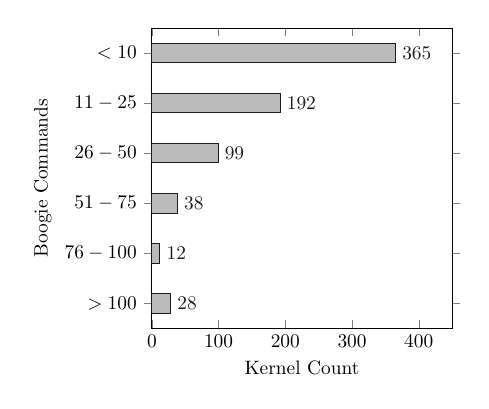
\begin{tikzpicture}[scale=0.7]
    
    \selectcolormodel{gray}
    
    \begin{axis}[
        xbar, xmin=0, xmax=450,
        xlabel={Kernel Count},
        symbolic y coords={
            {$> 100$},
            {$76-100$},
            {$51-75$},
            {$26-50$},
            {$11-25$},
            {$< 10$}
        },
        ytick=data,
        ylabel={Boogie Commands},
        nodes near coords,
        nodes near coords align={horizontal},
        height=200pt, width=200pt
    ]
    
    \addplot coordinates {
        (28,{$> 100$})
        (12,{$76-100$})
        (38,{$51-75$})
        (99,{$26-50$})
        (192,{$11-25$})
        (365,{$< 10$})
    };
    
    \end{axis}
    \end{tikzpicture}
    
    \caption{Boogie Commands}
    \label{Fi:boogie_commands}
\end{minipage}

\end{figure}


It should be noted that the instrumentation step of \tool happens on the Boogie code and not on the source code. A line of code in the source file could result in no Boogie commands (e.g., code comments) or more than one Boogie command (e.g., multiple assignments on a single line). \figref{boogie_commands} shows the size of the kernels in terms of Boogie commands. The average number of Boogie commands for the $734$ kernels for which Boogie code was generated was $25.72$, and the median was $11$. $50\%$ of the kernels had less than $25$ commands. The kernel with the highest number of Boogie commands had $1793$ commands.

\begin{figure}[htp]
\centering

\begin{minipage}{.45\textwidth}
    \centering
    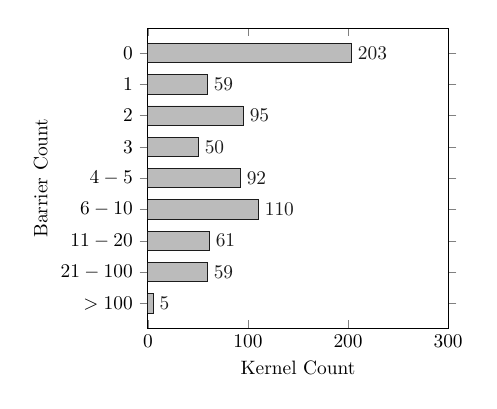
\begin{tikzpicture}[scale=0.7]
    
    \selectcolormodel{gray}
    
    \begin{axis}[
        xbar, xmin=0, xmax=300,
        xlabel={Kernel Count},
        symbolic y coords={
            {$> 100$},
            {$21-100$},
            {$11-20$},
            {$6-10$},
            {$4-5$},
            $3$,
            $2$,
            $1$,
            $0$
        },
        ytick=data,
        ylabel={Barrier Count},
        nodes near coords,
        nodes near coords align={horizontal},
        height=200pt, width=200pt
    ]
    
    \addplot coordinates {
        (5,{$> 100$})
        (59,{$21-100$})
        (61,{$11-20$})
        (110,{$6-10$})
        (92,{$4-5$})
        (50,$3$)
        (95,$2$)
        (59,$1$)
        (203,$0$)
    };
    
    \end{axis}
    \end{tikzpicture}
    
    \caption{Kernels with 'n' Instrumented Barriers}
    \label{Fi:kernels_barriers}
\end{minipage}

\end{figure}


The repair step of \tool does not depend on the number of lines or code nor the number of Boogie commands. It depends on the number of barriers that are instrumented in code which depend on the number of shared variables and how many times they have been used.

\figref{kernels_barriers} shows the number of barrier variables introduced in the instrumentation stage of \tool. This also includes the barrier variables introduced for existing barriers provided by the programmer. Out of the $734$ kernels that reached the instrumentation stage (inclusive of CUDA and OpenCL kernels), for $50\%$ of the kernels, the number of instrumented barriers introduced were less than or equal to $3$, whereas, there were $5$ kernels with more than $100$ instrumented barriers. For $50\%$ of the kernels, the time taken by the instrumentation stage of \tool was less than a second.

\section{Solver Comparison}

Besides the $mhs$ implementation of \tool, we introduce two more implementations of \tool, which use $MaxSAT$ and $SAT$ solvers, respectively, to solve the clauses. These implementations of \tool are used to repair all the $752$ kernels from \tableref{benchmark_summary}. \tableref{solver_comparison} summarizes the metrics of these three implementations. \figref{mhs_maxsat} and \figref{mhs_sat} show the time comparison between mhs and MaxSAT.

\begin{figure}[htp]
\centering
    \begin{tikzpicture}[scale=0.65]
    
    \pgfplotstableread{figures/data/time_mhs_maxsat.dat}{\data}
    \selectcolormodel{gray}
    
    \begin{axis}[
        xlabel={GPURepair (mhs)},
        ylabel={GPURepair (MaxSAT)},
        scaled ticks = false,
        tick label style={
            /pgf/number format/fixed,
            /pgf/number format/precision=3
        },
        xmin=1,
        xmax=300,
        ymin=1,
        ymax=300,
        xmode=log,
        ymode=log,
        log ticks with fixed point
    ]
    
    \addplot[
        scatter=true,
        only marks,
        mark=*,
        scatter src=explicit symbolic,
        scatter/classes={
            a={mark=*}
        }
    ]
    table[x=mhs,y=maxsat,meta=label]{\data};
    \addplot [black,samples at={0,1}] {x};
    \draw [black,solid] (rel axis cs:0,0) -- (rel axis cs:1,1);
    
    \end{axis}
    \end{tikzpicture}
    \caption{Runtime in seconds - mhs vs. MaxSAT (Log Scale)}
    \label{Fi:mhs_maxsat}
\end{figure}

\begin{table}[!h]
\caption{Solver Comparison}
\label{Ta:solver_comparison}
\begin{center}

\def\arraystretch{1.1}
\setlength\tabcolsep{7pt}

\begin{tabular}{|l|r|r|r|}
\hline

\multicolumn{1}{|c|}{} & \multicolumn{1}{|c|}{\textbf{mhs}} & \multicolumn{1}{|c|}{\textbf{MaxSAT}} & \multicolumn{1}{|c|}{\textbf{SAT}} \\ \hline \hline
Total Time Taken & $662$ & $662$ & $662$\\ \hline
Median Time Taken & $56$ & $662$ & $662$\\ \hline
Solver Calls & $8$ & $662$ & $662$\\ \hline
Verifier Calls & $26$ & $662$ & $662$\\ \hline

\end{tabular}

\end{center}
\end{table}


All three implementations repaired $83$ kernels ($53$ CUDA and $30$ OpenCL). \tableref{solver_comparison_repaired} summarizes the metrics of these three implementations for these repaired kernels.

\input{tables/solver_comparison_repaired}

\section{Configuration Comparison}

\tool provides the option of disabling instrumentation of grid-level barriers and disabling inspection of programmer inserted barriers. Disabling these configuration have a significant performance impact. By default both these options are enabled. These configuration options are used to repair all the $752$ kernels from \tableref{benchmark_summary}. \tableref{configuration_comparison} summarizes the metrics of these four configurations.

\section{Configuration Comparison}

\tool provides the option of disabling instrumentation of grid-level barriers and disabling inspection of programmer inserted barriers. Disabling these configuration have a significant performance impact. By default both these options are enabled. These configuration options are used to repair all the $@@kernel_count@@$ kernels from \tableref{benchmark_summary}. \tableref{configuration_comparison} summarizes the metrics of these four configurations.

\section{Configuration Comparison}

\tool provides the option of disabling instrumentation of grid-level barriers and disabling inspection of programmer inserted barriers. Disabling these configuration have a significant performance impact. By default both these options are enabled. These configuration options are used to repair all the $@@kernel_count@@$ kernels from \tableref{benchmark_summary}. \tableref{configuration_comparison} summarizes the metrics of these four configurations.

\section{Configuration Comparison}

\tool provides the option of disabling instrumentation of grid-level barriers and disabling inspection of programmer inserted barriers. Disabling these configuration have a significant performance impact. By default both these options are enabled. These configuration options are used to repair all the $@@kernel_count@@$ kernels from \tableref{benchmark_summary}. \tableref{configuration_comparison} summarizes the metrics of these four configurations.

\input{tables/configuration_comparison}

All four implementations give the same result for $@@same@@$ kernels ($@@same_cuda@@$ CUDA and $@@same_opencl@@$ OpenCL). \tableref{configuration_comparison_same} summarizes the metrics of these four configurations for these kernels.

\input{tables/configuration_comparison_same}


All four implementations give the same result for $@@same@@$ kernels ($@@same_cuda@@$ CUDA and $@@same_opencl@@$ OpenCL). \tableref{configuration_comparison_same} summarizes the metrics of these four configurations for these kernels.

\input{tables/configuration_comparison_same}


All four implementations give the same result for $@@same@@$ kernels ($@@same_cuda@@$ CUDA and $@@same_opencl@@$ OpenCL). \tableref{configuration_comparison_same} summarizes the metrics of these four configurations for these kernels.

\input{tables/configuration_comparison_same}


All four implementations give the same result for $83$ kernels ($53$ CUDA and $30$ OpenCL). \tableref{configuration_comparison_same} summarizes the metrics of these four configurations for these kernels.

\input{tables/configuration_comparison_same}
